\documentclass{beamer}

\usepackage[orientation=portrait, size=a0, scale=1.4]{beamerposter}

% \usetheme{confposter} % Use the confposter theme supplied with this template

\usepackage[utf8]{inputenc}
\usepackage[T1]{fontenc}
\usepackage[francais]{babel}

\usepackage{graphicx}
\usepackage{subfig}
\usepackage{xcolor}
\usepackage{enumitem}
\usepackage{wrapfig}

\definecolor{framebg}{RGB}{225, 225, 225}
\definecolor{titleboxbg}{RGB}{50, 205, 50}
\definecolor{bodyboxfg}{RGB}{75, 75, 75}

\setbeamertemplate{blocks}[rounded][shadow=false]
\setbeamertemplate{caption}[numbered]

\begin{document}
    \setbeamercolor{background canvas}{bg=framebg}
    \begin{frame}[t]
        %---------------------------
        %-          TITLE          -
        %---------------------------

        \setbeamercolor{block body}{fg=black,bg=titleboxbg} % Colors of the block titles
        \begin{block}{}
            \begin{columns}[t]
                \begin{column}{.1\linewidth}
                    \begin{figure}[t]
                        
\includegraphics[width=\linewidth]{rsc/logo_um.png}
                    \end{figure}
                \end{column}

                \begin{column}{.75\linewidth}
                    \begin{center}
                        {\Huge \textbf{Musée sécurisé en réalité augmentée}}
                    \end{center}

                    \begin{columns}[t]
                        \begin{column}{.5\linewidth}
                            \begin{center}
                                \textbf{Présenté par\\Théo Clayette, Thibaut Etienne, Arnaud Soulier}
                            \end{center}
                        \end{column}

                        \begin{column}{.5\linewidth}
                            \begin{center}
                                \textbf{Sous la direction de\\William Puech, Pauline Puteaux}
                            \end{center}
                        \end{column}
                    \end{columns}
                \end{column}

                \begin{column}{.1\linewidth}
                    \begin{figure}[t]
                        
\includegraphics[width=\linewidth]{rsc/logo_lirmm.png}
                    \end{figure}
                \end{column}
            \end{columns}
        \end{block}

        %----------------------------
        %-          POSTER          -
        %----------------------------

        \begin{columns}[t]
            %------------------------------------------
            %-          POSTER - CHIFFREMENT          -
            %------------------------------------------

            \begin{column}{.49\linewidth}

                %--------------------------------
                %-          C1 - INDEX          -
                %--------------------------------

                \setbeamercolor{block title}{fg=white,bg=titleboxbg} % Colors of the block titles
                \setbeamercolor{block body}{fg=bodyboxfg,bg=white} % Colors of the block titles
                \begin{block}{\centering \textbf{Chiffrement - Méthode}}
                    \vspace{0.5cm}

                    \begin{figure}[t]
                        \begin{center}
                            \captionsetup[subfigure]{justification=centering}
                            \subfloat[Itération 1]{
                                
\includegraphics[width=.3\linewidth]{rsc/index_1.png}}
                            \subfloat[Itération 2]{
                                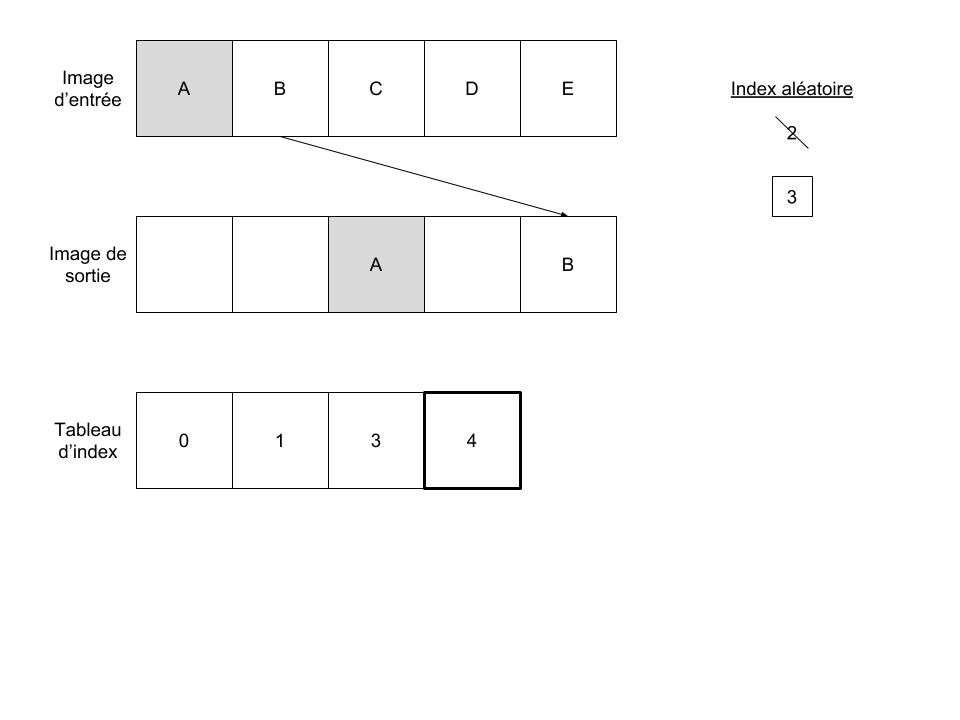
\includegraphics[width=.3\linewidth]{rsc/index_2.png}}
                            \subfloat[Itération 3]{
                                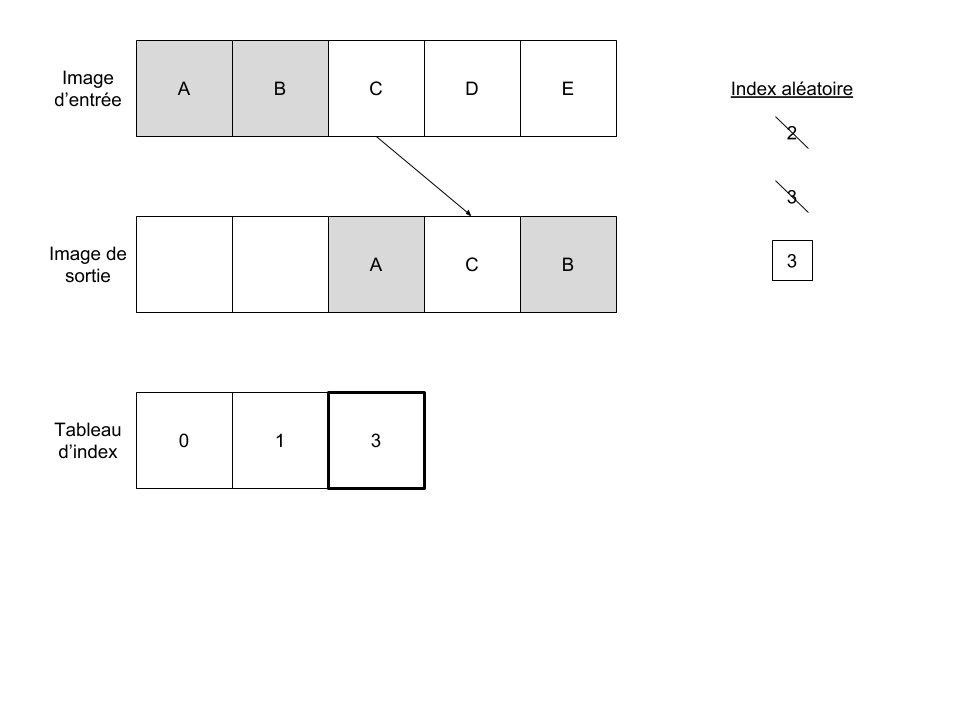
\includegraphics[width=.3\linewidth]{rsc/index_3.png}}
                            \caption{\centering Algorithme de chiffrement pseudo-aléatoire}
                        \end{center}
                    \end{figure}

                    Chaque itération se décompose en 4 étapes :
                    \begin{itemize}[label=-]
                        \item Tirage d'un nombre aléatoire $r$ entre 0 et la taille d'un tableau d'index.
                        \item Récupération du nouvel indice $n$ du pixels dans le tableau d'index à l'indice $r$.
                        \item Écriture du pixels dans la nouvelle case $n$ de l'image de sortie.
                        \item Suppression de la case $n$ du tableau d'index.
                    \end{itemize}

                    \vspace{0.5cm}
                \end{block}



                %------------------------------------
                %-          C1 - Résultats          -
                %------------------------------------

                \setbeamercolor{block title}{fg=white,bg=titleboxbg} % Colors of the block titles
                \setbeamercolor{block body}{fg=bodyboxfg,bg=white} % Colors of the block titles
                \begin{block}{\centering \textbf{Chiffrement - Résultats}}
                    \vspace{0.5cm}

                    \begin{figure}[t]
                        \begin{center}
                            \captionsetup[subfigure]{justification=centering}
                            \subfloat[Image original de 800x800 pixels]{
                                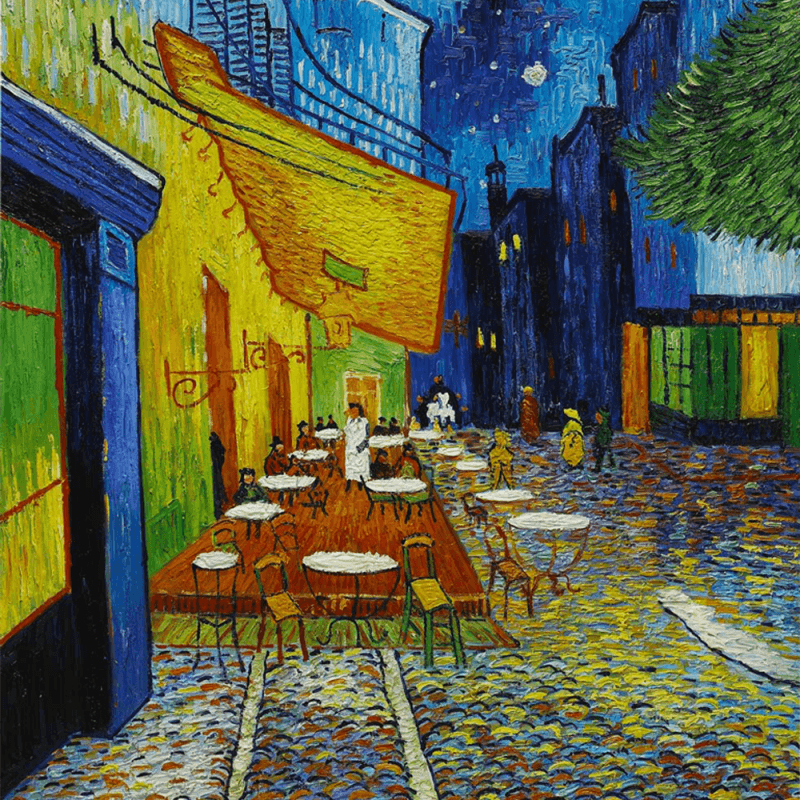
\includegraphics[width=.185\linewidth]{rsc/van_gogh.png}}
                            \hspace{.1\linewidth}
                            \subfloat[Chiffrement par 800x800 blocs de 1x1 pixels]{
                                
\includegraphics[width=.185\linewidth]{rsc/van_gogh_800.png}}\\
                            \subfloat[Chiffrement par 10x10 blocs de 80x80 pixels]{
                                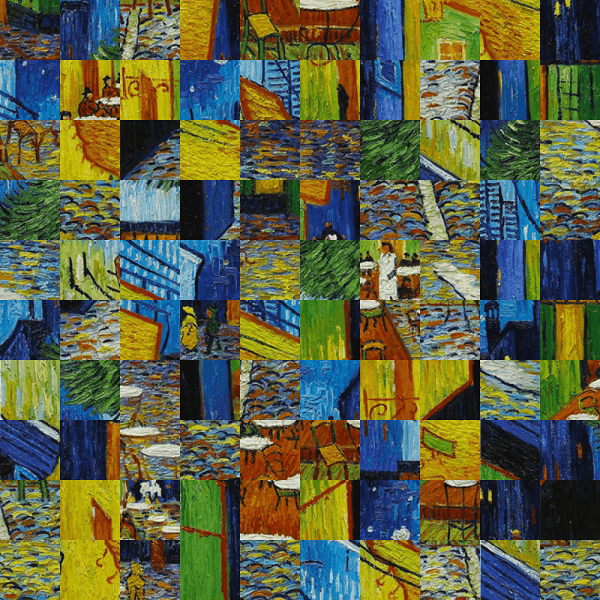
\includegraphics[width=.185\linewidth]{rsc/van_gogh_10.png}}
                            \hspace{.1\linewidth}
                            \subfloat[Chiffrement par 25x25 blocs de 32x32 pixels]{
                                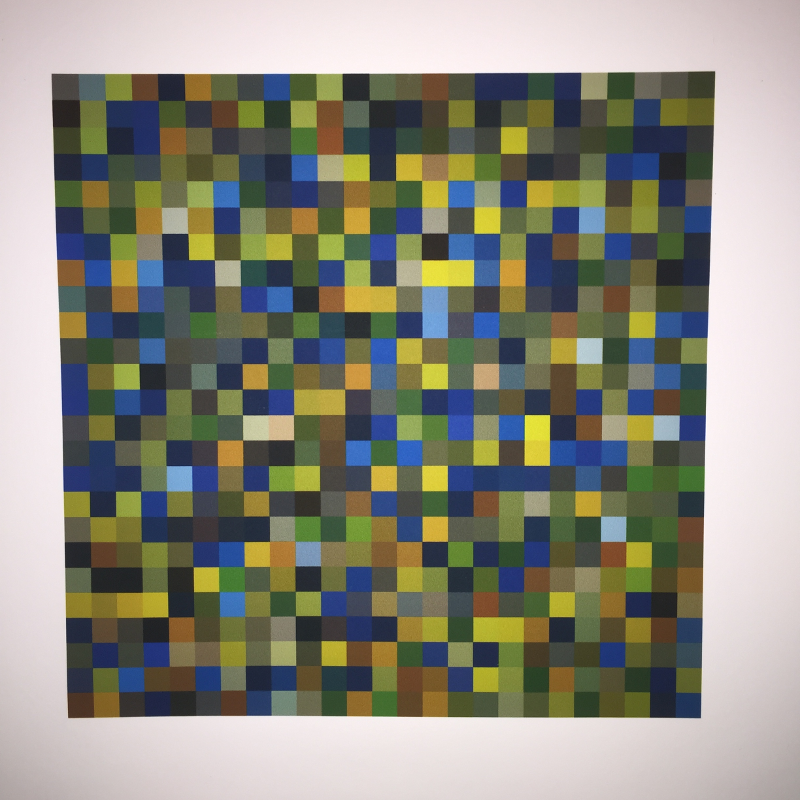
\includegraphics[width=.185\linewidth]{rsc/van_gogh_25.png}}
                            \hspace{.1\linewidth}
                            \subfloat[Chiffrement par 50x50 blocs de 16x16 pixels]{
                                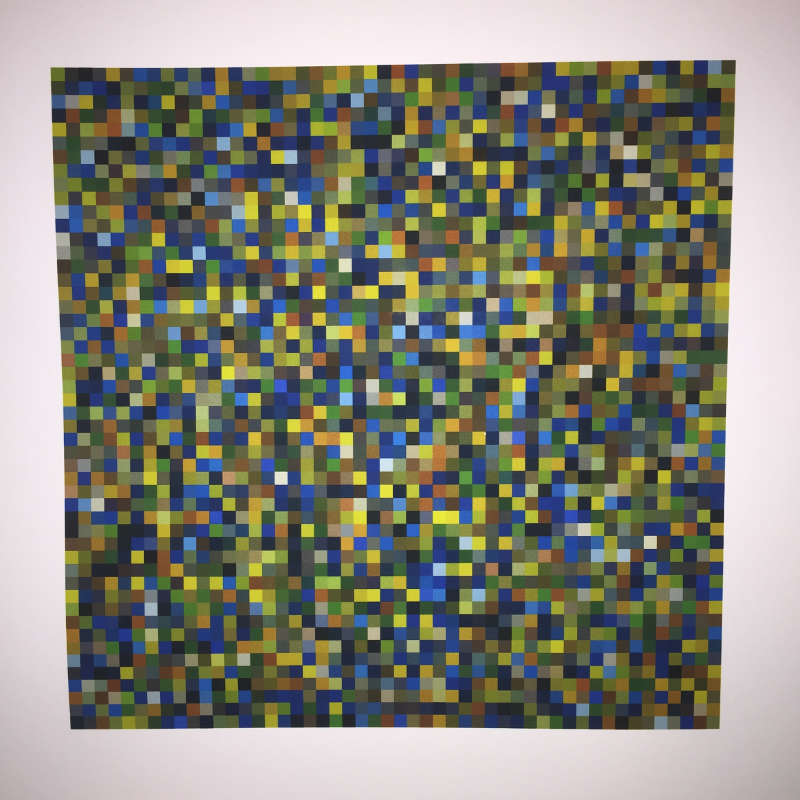
\includegraphics[width=.185\linewidth]{rsc/van_gogh_50.png}}\\
                            \subfloat[Chiffrement par 10x10 blocs de 80x80 pixels moyennés]{
                                
\includegraphics[width=.185\linewidth]{rsc/van_gogh_10_a.png}}
                            \hspace{.1\linewidth}
                            \subfloat[Chiffrement par 25x25 blocs de 32x32 pixels moyennés]{
                                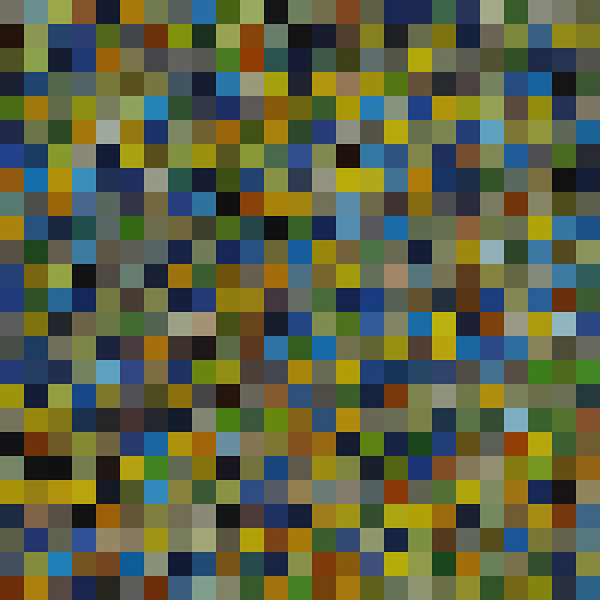
\includegraphics[width=.185\linewidth]{rsc/van_gogh_25_a.png}}
                            \hspace{.1\linewidth}
                            \subfloat[Chiffrement par 50x50 blocs de 16x16 pixels moyennés]{
                                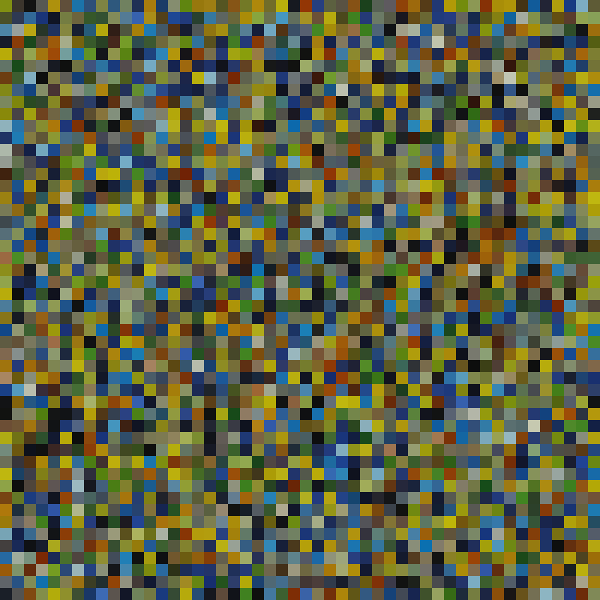
\includegraphics[width=.185\linewidth]{rsc/van_gogh_50_a.png}}\\
                            \caption{\centering Chiffrement par bloc et bloc moyenné de la "Térasse du café le soir" de Van Gogh}
                        \end{center}
                    \end{figure}

                    \vspace{0.5cm}
                \end{block}



                %-----------------------------------------------
                %-          C2 - QUALITE RESSEMBLANCE          -
                %-----------------------------------------------

                \setbeamercolor{block title}{fg=white,bg=titleboxbg} % Colors of the block titles
                \setbeamercolor{block body}{fg=bodyboxfg,bg=white} % Colors of the block titles
                \begin{block}{\centering \textbf{Qualité de ressemblance de l'oeuvre}}
                    \vspace{0.5cm}

                    \begin{center}
                        \begin{figure}[t]
                            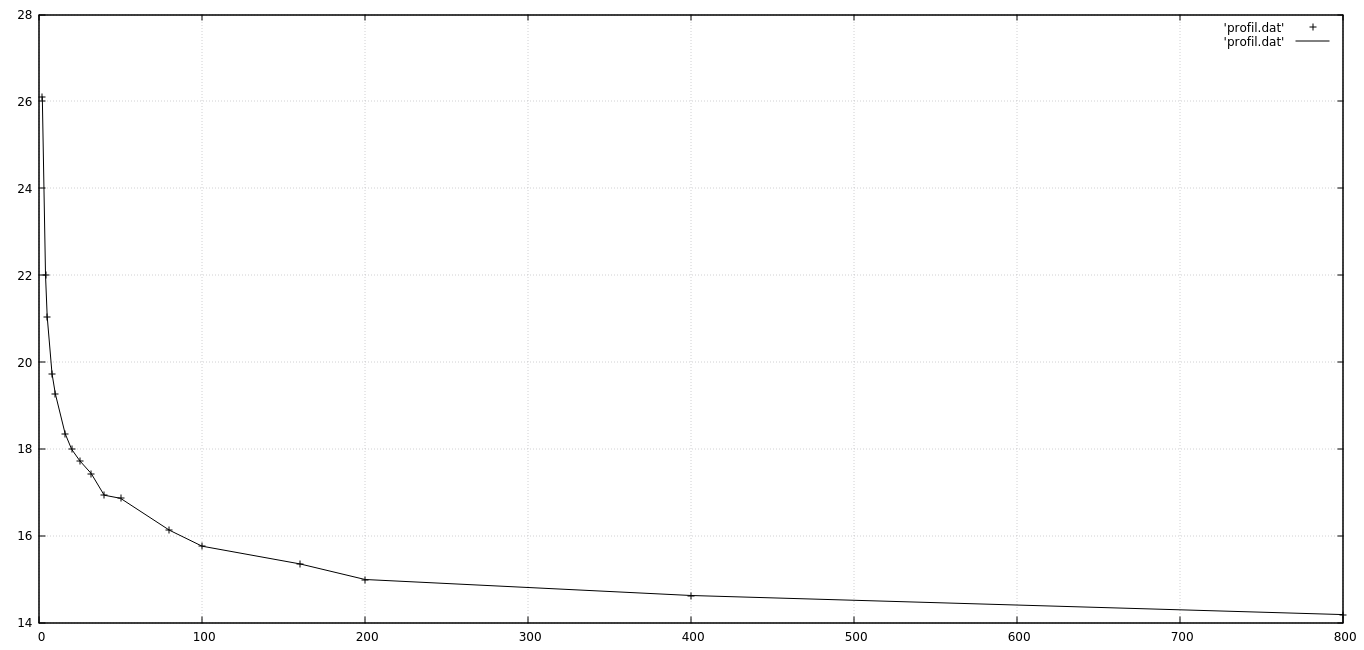
\includegraphics[width=.5\linewidth]{rsc/psnr_ressemblance.png}
                            \caption{\centering PSNR de la peinture en fonction de la taille des blocs}
                        \end{figure}
                    \end{center}

                    D'après le PSNR (Peak Signal to Noise Ratio) obtenu avec le découpage en bloc de diverses tailles de la peinture, on observe une qualité acceptable (PSNR >= 20 db) à partir d'une taille de bloc de 8x8 pixels (19.6387 db).
                    Toutes les décompositions avec des blocs d'une taille inférieure ou égale à 8x8 pixels sont donc considéré comme ressemblante à l'oeuvre d'origine.

                    \vspace{0.5cm}
                \end{block}



                %----------------------------------------
                %-          C2 - PRETRAITEMENT          -
                %----------------------------------------

                \setbeamercolor{block title}{fg=white,bg=titleboxbg} % Colors of the block titles
                \setbeamercolor{block body}{fg=bodyboxfg,bg=white} % Colors of the block titles
                \begin{block}{\centering \textbf{Lecture - Prétraitements}}
                    \vspace{0.5cm}

                    Traitement à effectuer sur la photo pour permettre la transformation :
                    \begin{itemize}[label=\textbullet]
                        \item Conversion en image en niveau de gris :
                        \begin{itemize}[label=$\rightarrow$]
                            \item 0.299 $\cdot$ rouge + 0.587 $\cdot$ vert + 0.114 $\cdot$ bleu.
                        \end{itemize}
                        \item Conversion en image binaire :
                        \begin{itemize}[label=$\rightarrow$]
                            \item seuil avec la variance moyenne pour séparer la peinture du fond pour failiter la détection des angles.
                        \end{itemize}
                        \item Détection des angles :
                        \begin{itemize}[label=$\rightarrow$]
                            \item trouve les quatres points tels que leurs distances aux coins respectifs de l'image soit minimale.
                        \end{itemize}
                        \item Balance des blancs :
                        \begin{itemize}[label=$\rightarrow$]
                            \item ajuste les couleurs pour se rapprocher des couleurs réelles.
                        \end{itemize}
                    \end{itemize}

                    \vspace{0.5cm}
                \end{block}
            \end{column}

            %--------------------------------------------
            %-          POSTER - DECHIFFREMENT          -
            %--------------------------------------------

            \begin{column}{.49\linewidth}

                %----------------------------------------
                %-          C2 - TRANFORMATION          -
                %----------------------------------------

                \setbeamercolor{block title}{fg=white,bg=titleboxbg} % Colors of the block titles
                \setbeamercolor{block body}{fg=bodyboxfg,bg=white} % Colors of the block titles
                \begin{block}{\centering \textbf{Lecture - Transformation}}
                    \vspace{0.5cm}

                    \begin{wrapfigure}[6]{l}{.4\linewidth}
                        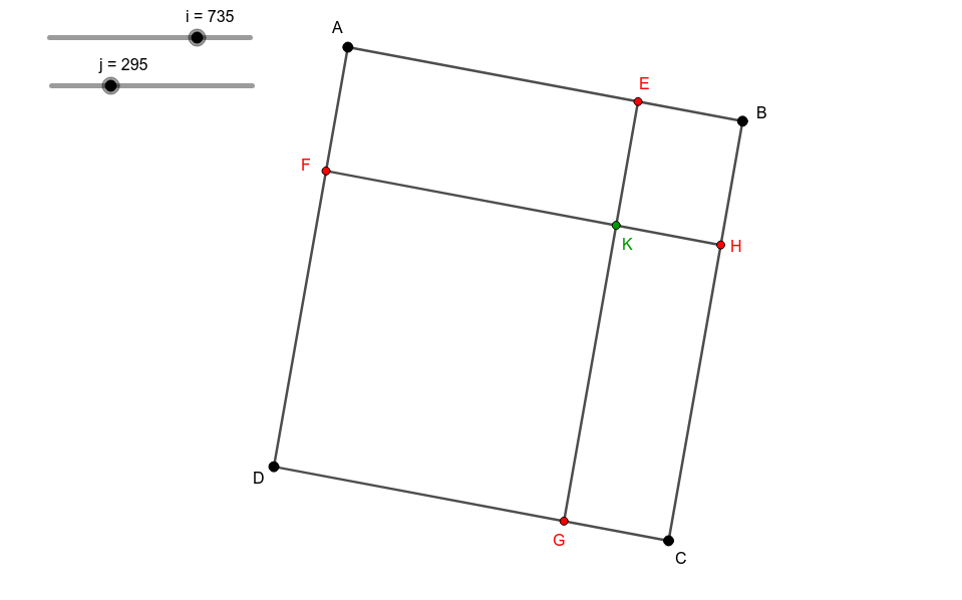
\includegraphics[width=\linewidth]{rsc/formule_transformation.png}
                    \end{wrapfigure}
                    L'opération effectué pour obtenir l'image de la peinture pour le déchiffrement associe une transformation affine ainsi qu'une interpolation.
                    Les quatre angles de la peinture définissent les points A, B, C et D. Les points E, F, G et H se déplace respectivement sur les segments AB, AD, DC et BC. Le point K est l'intersection entre les segments EG et FH.
                    L'image que l'on souhaite écrire est parcouru selon ses x et ses y et le pixels lu correspond au coordoonées du point K. Les coordonnées de E, F, G et H sont calculé en fonction de ces x et y ainsi que le la taille de l'image de sortie voulue.

                    \vspace{0.5cm}
                \end{block}

                %------------------------------------
                %-          C2 - RESULTATS          -
                %------------------------------------

                \setbeamercolor{block title}{fg=white,bg=titleboxbg} % Colors of the block titles
                \setbeamercolor{block body}{fg=bodyboxfg,bg=white} % Colors of the block titles
                \begin{block}{\centering \textbf{Lecture - Résultats}}
                    \vspace{0.5cm}

                    \begin{figure}[t]
                        \begin{center}
                            \captionsetup[subfigure]{justification=centering}
                            \subfloat[Photo 10x10 blocs de 80x80 pixels]{
                                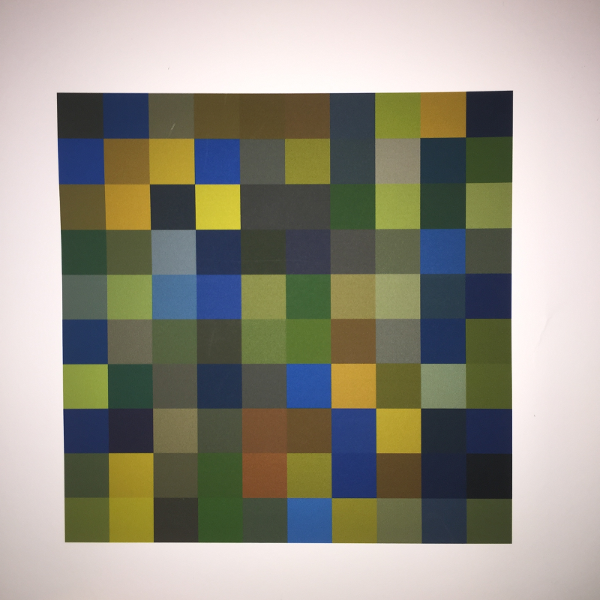
\includegraphics[width=.25\linewidth]{rsc/van_gogh_10_p.png}}
                            \hspace{.05\linewidth}
                            \subfloat[Photo 40x40 blocs de 20x20 pixels]{
                                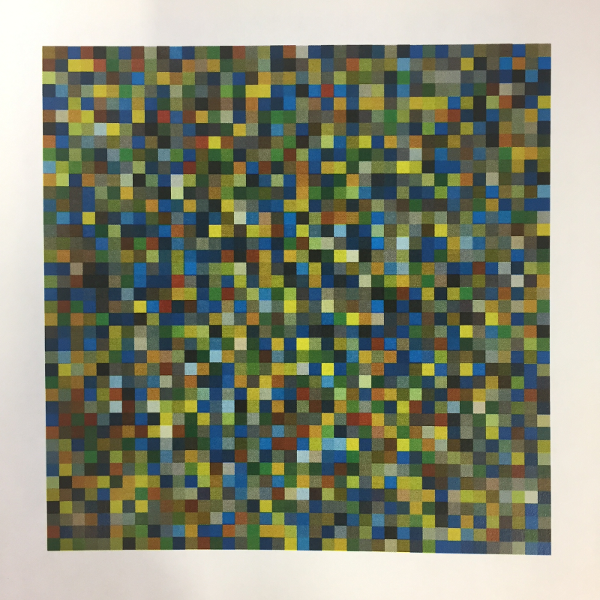
\includegraphics[width=.25\linewidth]{rsc/van_gogh_40_p.png}}
                            \hspace{.05\linewidth}
                            \subfloat[Photo 50x50 blocs de 16x16 pixels]{
                                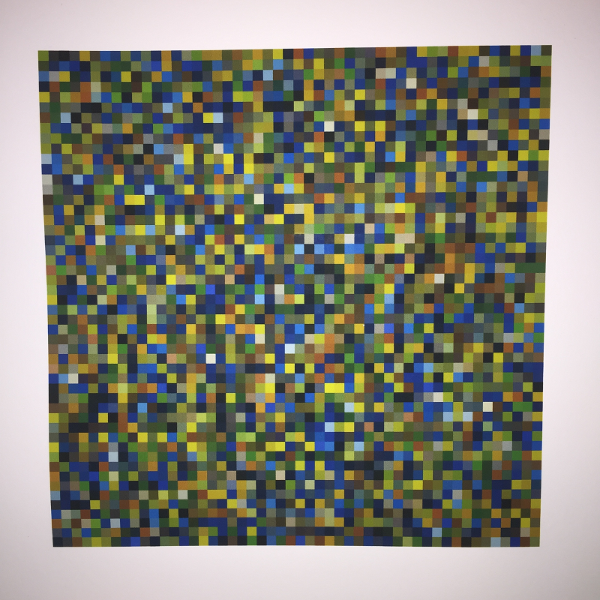
\includegraphics[width=.25\linewidth]{rsc/van_gogh_50_p.png}}\\
                            \subfloat[Déchiffrement par 10x10 blocs de 80x80 pixels]{
                                
\includegraphics[width=.25\linewidth]{rsc/van_gogh_10_d_a.png}}
                            \hspace{.05\linewidth}
                            \subfloat[Déchiffrement par 40x40 blocs de 20x20 pixels]{
                                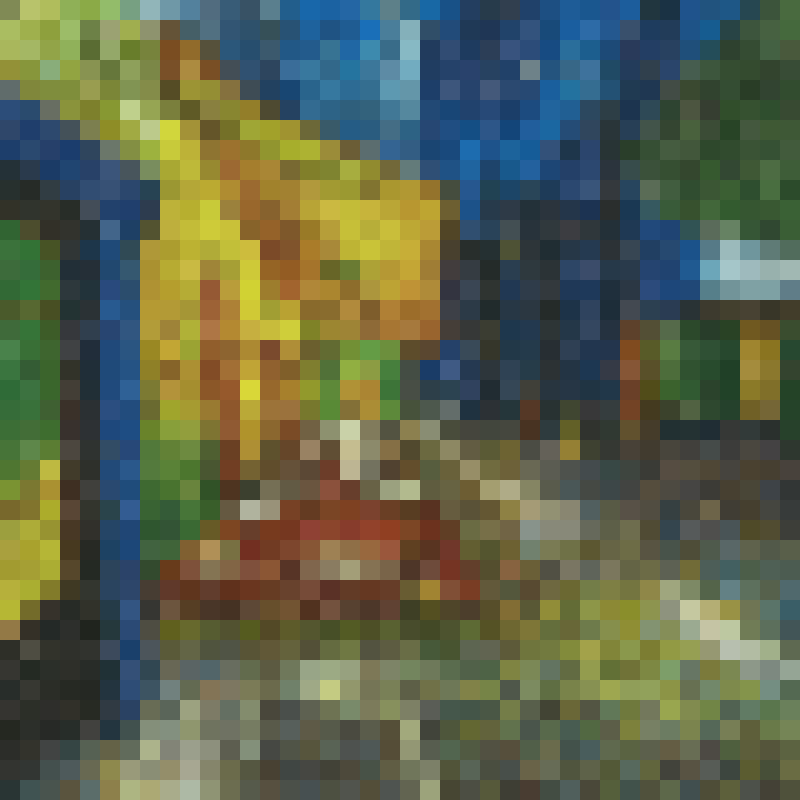
\includegraphics[width=.25\linewidth]{rsc/van_gogh_40_d_a.png}}
                            \hspace{.05\linewidth}
                            \subfloat[Déchiffrement par 50x50 blocs de 16x16 pixels]{
                                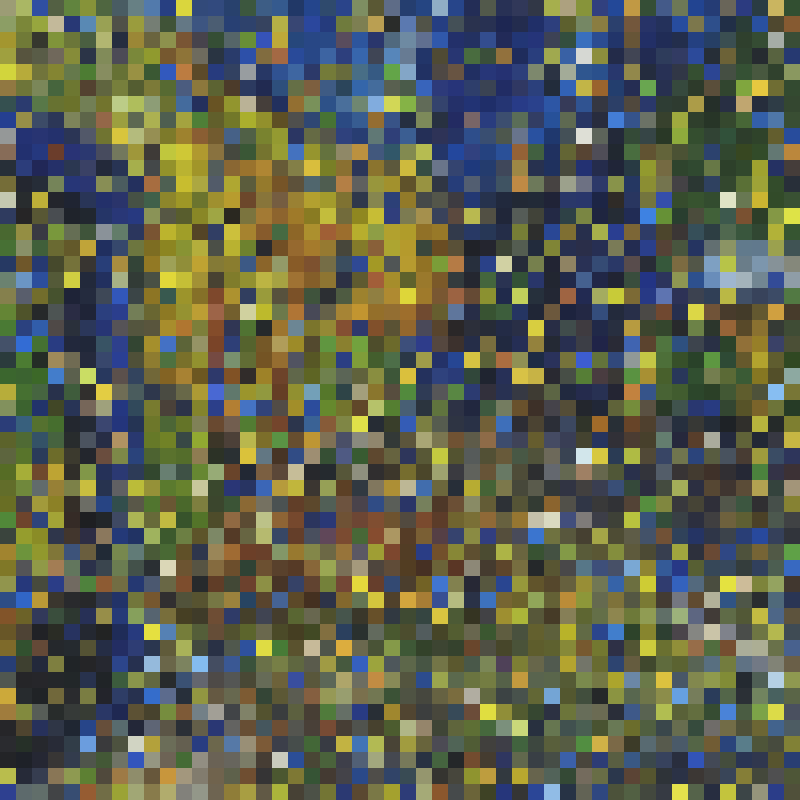
\includegraphics[width=.25\linewidth]{rsc/van_gogh_50_d_a.png}}\\
                            \caption{\centering Lecture et déchiffrement par bloc moyenné de la "Térasse du café le soir" de Van Gogh}
                        \end{center}
                    \end{figure}

                    Comme le montre ces résultats, le déchiffrement des peintures imprimées est plus ou moins efficace en fonction de la taille de bloc utilisé pendant la phase de chiffrement.
                    \begin{itemize}[label=-]
                        \item pour une taille 80x80, le déchiffrement est fonctionnel mais le résultat n'est pas reconnaissable
                        \item pour une taille 20x20, le déchiffrement reste fonctionnel et le résultat est lisible même s'il présente du bruit
                        \item pour une taille de 16x16, le déchiffrement n'est plus fonctionnel et le résultat n'est plus lisible
                    \end{itemize}

                    \vspace{0.5cm}
                \end{block}

                %------------------------------------------
                %-          C2 - QUALITE LECTURE          -
                %------------------------------------------

                \setbeamercolor{block title}{fg=white,bg=titleboxbg} % Colors of the block titles
                \setbeamercolor{block body}{fg=bodyboxfg,bg=white} % Colors of the block titles
                \begin{block}{\centering \textbf{Qualité de lecture de l'oeuvre imprimée}}
                    \vspace{0.5cm}

                    \begin{center}
                        \begin{figure}[t]
                            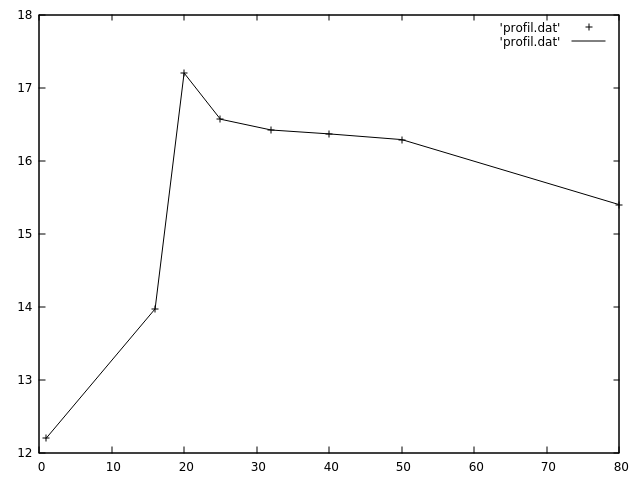
\includegraphics[width=.5\linewidth]{rsc/psnr_lecture.png}
                            \caption{\centering PSNR de la lecture de la peinture en fonction de la taille des blocs}
                        \end{figure}
                    \end{center}

                    La qualité d'acquisition de l'image dépend de l'appareil utilisé. Dans le cadre de ce projet, il s'agit d'un Iphone 6.
                    Plus la taille des blocs est petite, plus la peinture déchiffré est ressemblante à l'oeuvre d'origine. Cependant, si l'on atteint la taille de 16x16 pixels, la précision de l'image est trop grande pour permettre un déchiffrement correct de la peinture.
                    Le meilleur résultat obtenable avec cet appareil est avec un découpage en blocs de maximum 20x20 pixels.
                    La point de chute pour une taille de 32x32 pixels est dû à la différence de la qualité de la prise de photo (cadrage, plassement au centre, lumière, etc...).

                    \vspace{0.5cm}
                \end{block}
            \end{column}
        \end{columns}
    \end{frame}
\end{document}
